%! TeX program = lualatex
\documentclass[a4paper]{article}

\usepackage{multicol}

% packages
\usepackage{microtype}      % Slightly tweak font spacing for aesthetics
\usepackage[english]{babel} % Language hyphenation and typographical rules
\usepackage[final, colorlinks = true, allcolors=black]{hyperref}
\usepackage{changepage}     % adjust margins on the fly

\usepackage{fontspec}
\setmainfont{EB Garamond}
\setmonofont[Scale=MatchLowercase]{Deja Vu Sans Mono}

\usepackage{minted}
\usemintedstyle{algol_nu}
\usepackage{xcolor}

\usepackage{pgfplots}
\pgfplotsset{width=\textwidth,compat=1.9}

\usepackage{caption}
\newenvironment{code}{\captionsetup{type=listing}}{}
\captionsetup[listing]{skip=0pt}
\setlength{\abovecaptionskip}{5pt}
\setlength{\belowcaptionskip}{5pt}

\usepackage[yyyymmdd]{datetime}
\renewcommand{\dateseparator}{--}

\usepackage[backend=bibtex, style=numeric, sorting=none]{biblatex}
\bibliography{references}

\usepackage{titlesec}

% margins
\addtolength{\hoffset}{-2.25cm}
\addtolength{\textwidth}{4.5cm}
\addtolength{\voffset}{-3.25cm}
\addtolength{\textheight}{5cm}
\setlength{\parskip}{0pt}
\setlength{\parindent}{0in}

\begin{document}
\hrule \medskip
\begin{minipage}{0.295\textwidth}
    \raggedright
    \footnotesize
    Name: Andrew Hayes \\
    E-mail: \href{mailto://a.hayes18@universityofgalway.ie}{\texttt{a.hayes18@universityofgalway.ie}}  \hfill\\
    ID: 21321503 \hfill
\end{minipage}
\begin{minipage}{0.4\textwidth}
    \centering
    \vspace{0.4em}
    \Large
    \textbf{CT3112} \\
\end{minipage}
\begin{minipage}{0.295\textwidth}
    \raggedleft
    \today
\end{minipage}
\medskip\hrule
\begin{center}
    \normalsize
    Professional Skills: Health \& Safety Assignment
\end{center}
\hrule

\begin{figure}[h]
    \centering
    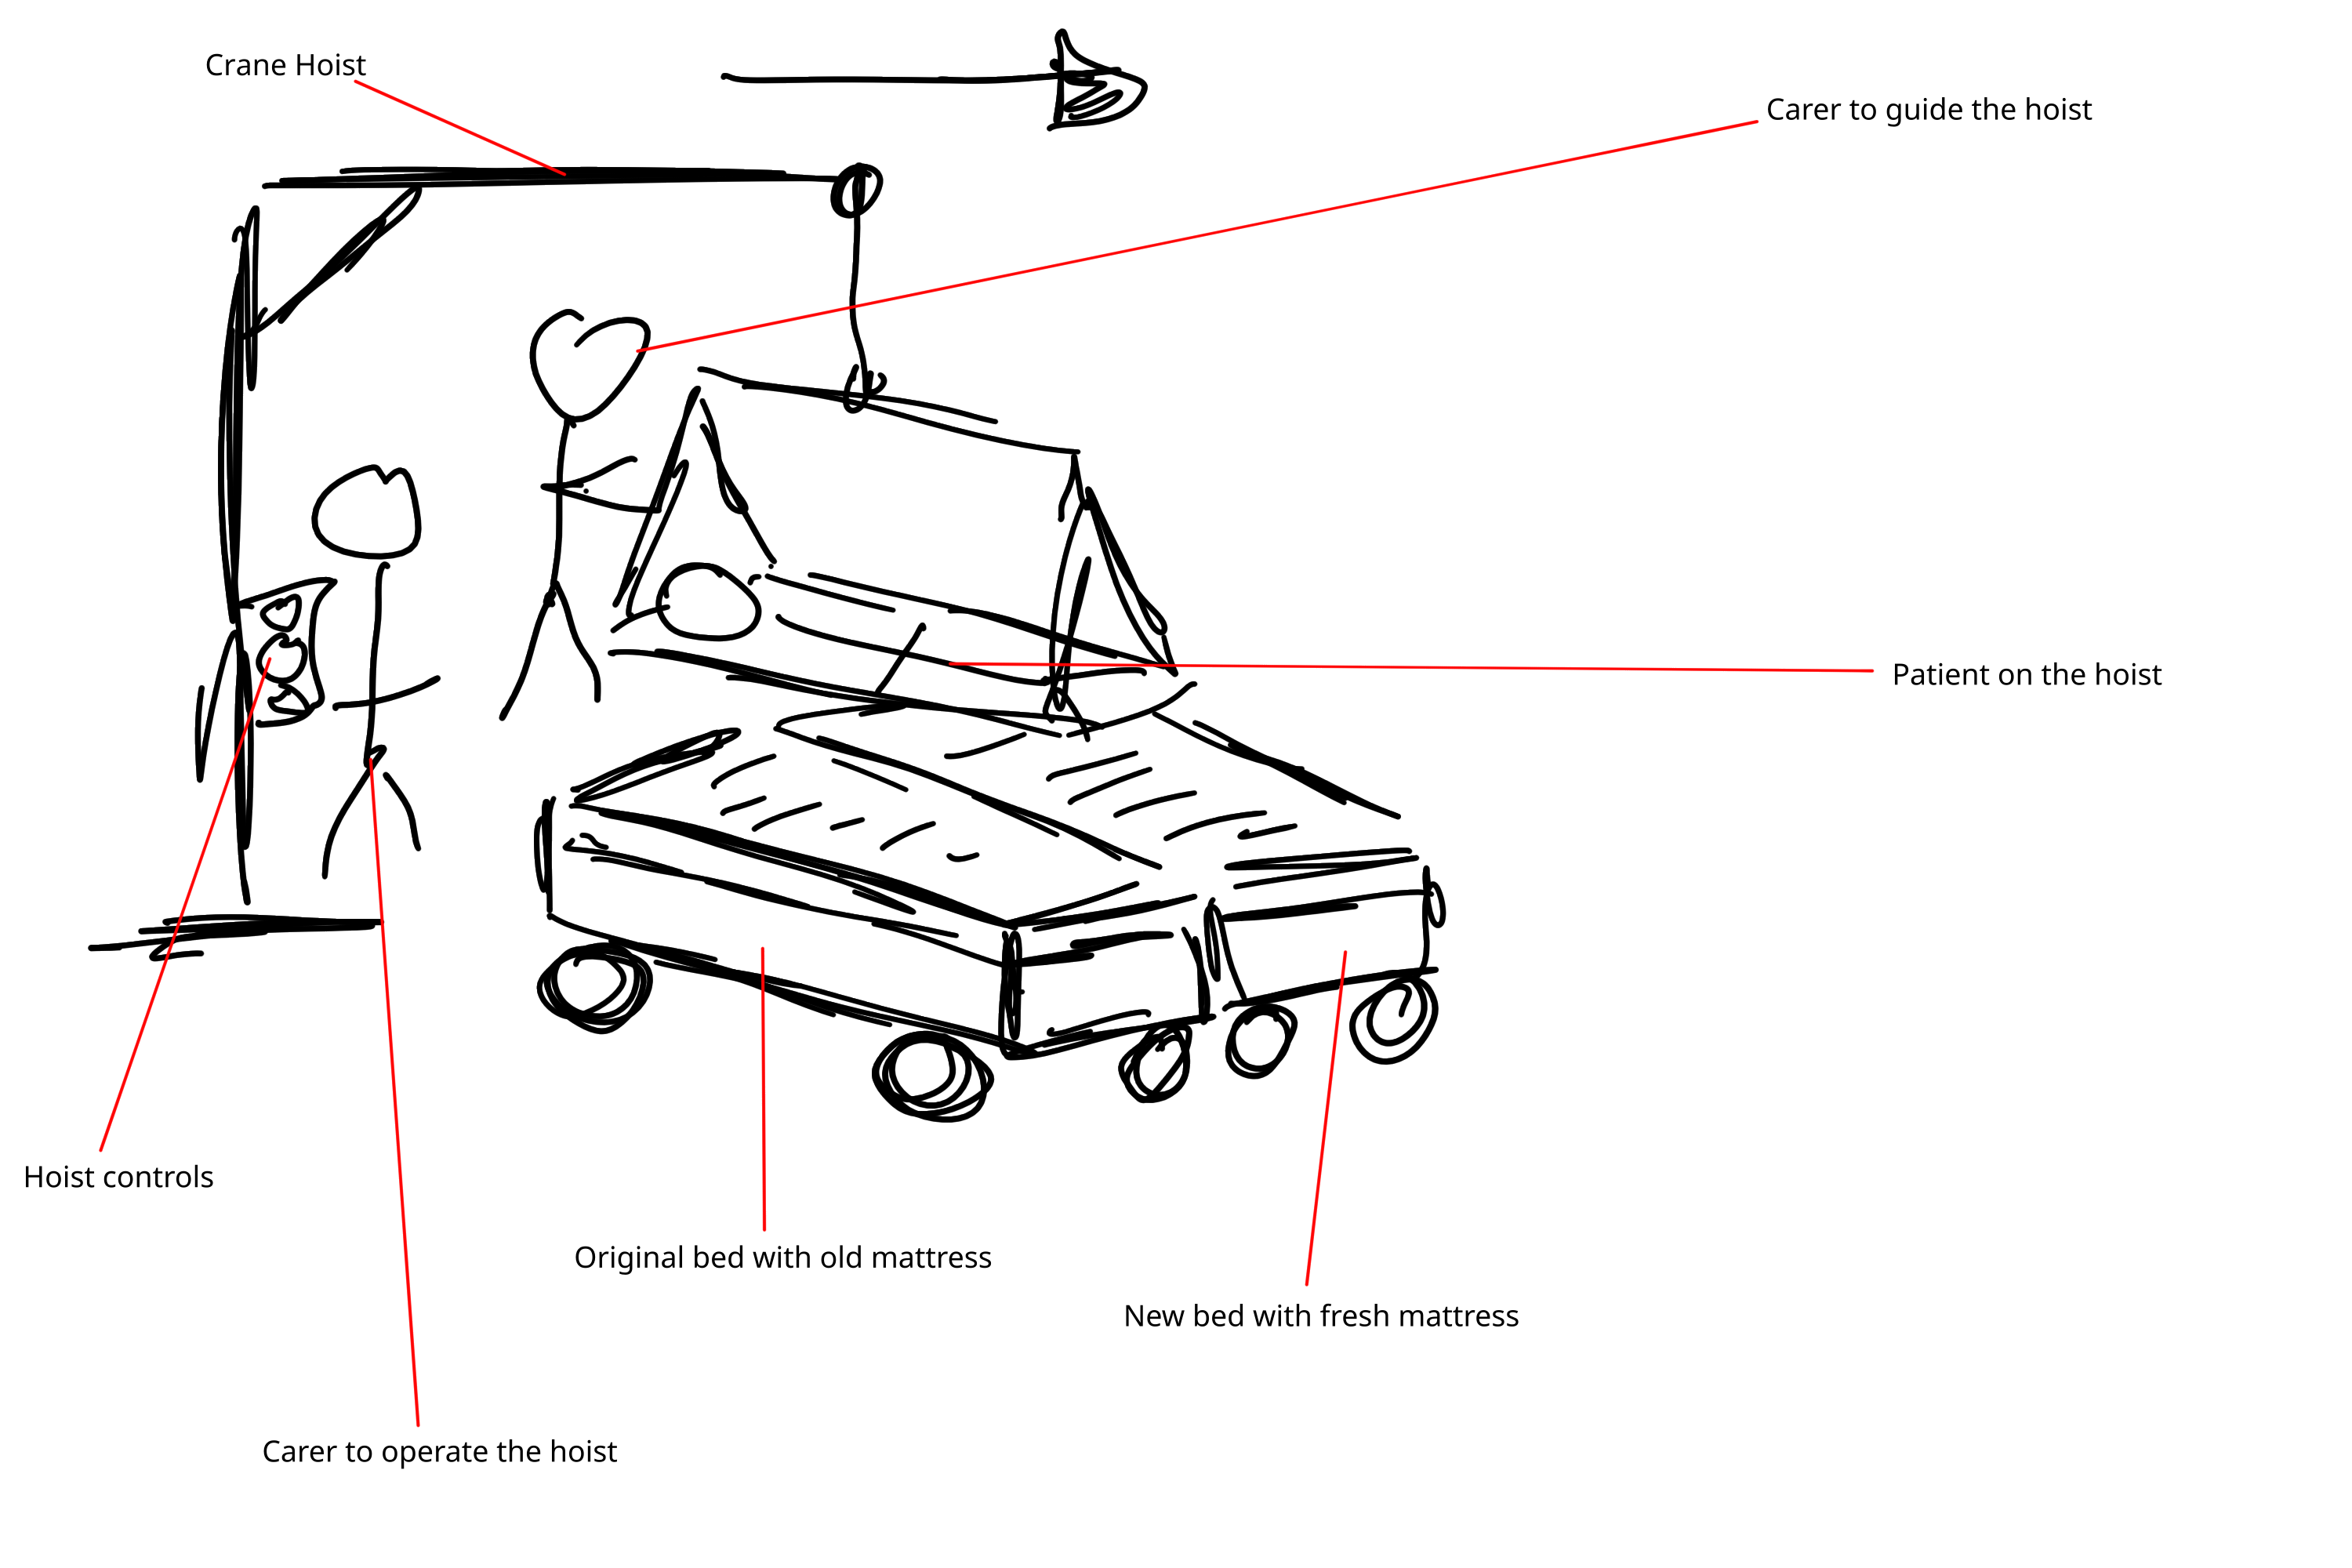
\includegraphics[width=0.50\textwidth]{sketch.png}
    \caption{Sketch}
\end{figure}


\begin{multicols}{2}
\section{Chosen Video}
I have chosen the ``\href{https://www.youtube.com/watch?v=RF6PrPhyoXs}{Patient Full Body Lift Case Study}''
video from the
\href{https://www.hsa.ie/eng/Workplace_Health/Manual_Handling_Display_Screen_Equipment/Risk_Assessment_Videos/Manual_Handling_Videos_Series_2/}{Manual Handling Video Series 2} for this assignment.

\section{Novel Risk Control Strategy}
My proposed novel alternative risk control strategy involves introducing a second trolley bed.
A second trolley bed would be prepared with a fresh mattress, and placed alongside the patient's current bed, thus
minimising the travel distance.
The patient should then be moved from the old bed to the new bed in whichever manner is safest \& least likely to cause
injury for both the patient \& the carers.
If the patient is physically capable, they should move themselves from the old bed to the new, either by getting up and
walking around or rolling over from one to the other.
Otherwise, if the patient is not able to safely move themselves from the old bed to the new, they should be hoisted
with a crane hoist from the old bed to the new, with one carer operating the hoist and another carer guiding the hoist,
ensuring that it doesn't swing and hurt either a carer or the patient.
The trolley wheel brakes of both beds should be applied before any movement is undertaken to prevent either of the beds
from slipping and causing an accident.
\\\\
Once the patient has been moved from the old bed to the new, the mattress from the old bed can then be removed by a
carer and disposed of as suitable.
The use of two beds does add the required extra component of an empty and available trolley, but this is a small price
to pay for a more safe \& reliable procedure.
\\\\
The carers should be trained in this procedure so that they can do it easily \& with familiarity, and they should also
be trained on the operation of the hoist crane if they have not been previously.

\subsection{How are the Specific Hazards \& Risks Identified in the Video Addressed?}
\subsubsection{Individual's weight outside the guidelines}
\label{sec:weight-outside-guidelines}
The problem of the patient being too heavy for the carers to safely lift themselves is eliminated by the use of a
bariatric medical hoist which can hold up to 400kg \supercite{optomed} safely, and any potential injuries incurred by
the carers from the strain can be avoided.
The high weight capacity of the hoist means that the patient's weight should never exceed the weight guidelines.
Furthermore, this also eliminates risks of the patient being dropped by the carers if they are not strong enough to hold
the patient for the prolonged period, avoiding potential injuries to the patient.

\subsubsection{Physical Effort is Too Strenuous}
The problem of the physical effort being to strenuous for the carers is eliminated by the use of hoist, much in the same
manner as outlined above in the \textbf{\nameref{sec:weight-outside-guidelines}} section, as the need for physical
effort from the carers is eliminated. 
Even the disposing of the mattress can be done with less effort on the part of the carers as it's on a trolley that can
be moved easily.
There is also no need to rapidly move the mattresses on \& off the bed, further reducing strain.

\subsubsection{Body in an unstable posture}
Again, the use of the hoist eliminates the problem of the carers' bodies being in unstable postures.
The uneven strain on the patient's body from being lifted by several carers is eliminated by the use of hoist that
distributes their weight evenly.

\subsubsection{Sudden movement of the load}
The use of the hoist eliminates the problem of the load undergoing sudden movement, as it can be lifted slowly \&
gently -- there is no ``heaving'' movement.

\subsubsection{Prolonged physical effort}
The use of the hoists and the trolleys eliminates all physical effort for the carers, prolonged or otherwise.

\subsubsection{Uncoordinated lift}
The hoist eliminates the problem of the lift being uncoordinated by eliminating the need for coordination between the
carers lifting the patient. 
Since there is only one mechanism lifting the patient (the hoist), there is no need to coordinate between different
lifters.

\subsubsection{Patient handled at a distance from the trunk of the carers' bodies}
Since the carers are not lifting the patient themselves, the problem of the patient being handled at a distance from the
trunk of their bodies is eliminated.

\subsection{How does the Strategy Comply with the General Principles of Prevention?\supercite{isb}}
\subsubsection{The avoidance of risks.}
The strategy avoids the risk incurred by the manual lifting of the patient by replacing it with a more reliable hoist
system.
In the event that the patient is capable of moving themselves, the risks associated with lifting the patient are avoided
entirely, thus making this strategy highly avoidant to risks.

\subsubsection{The evaluation of unavoidable risks.}
If the patient is unable to move themselves from one bed to the next, there is the unavoidable risk of the hoist
undergoing a mechanical failure and dropping the patient, potentially injuring the patient or the carers.
Since this risk cannot be entirely eliminated, the carers should be trained on how to try and avoid the risk and how to
deal with the aftermath of a mechanical failure of the hoist.
The carers should check the weight of the patient and the weight limit of the hoist before undertaking the procedure,
and should conduct an inspection of the hoist to ensure that it is in working order beforehand.
All carers should stand a safe distance from the hoist when it is in operation, and the patient should only be moved
over the beds so that if they are dropped they land on a soft, elevated surface.

\subsubsection{The combating of risks at source.}
The majority of the risks involved with the original technique stemmed from the manual lifting of the patient. 
This is combatted at the source by removing the need for manual lifting.

\subsubsection{The adaptation of work to the individual, especially as regards the design of places of work, the choice of work equipment, \& the choice of systems of work, with a view, in particular, to alleviating monotonous work and work at a predetermined work rate and to reducing the effect of this work on health.}
Monotonous work is avoided by greatly speeding up the procedure.
The effect of the work on the health of the carer is minimised by eliminating the physical strain \& labour they have to
undergo.

\subsubsection{The adaptation of the place of work to technical progress.}
The strategy complies with the principle of the adaptation of the place of work to technical progress by replacing the
more primitive method of moving a patient (manually lifted by the carers) by a more technologically advanced method
(lifting with a hoist).

\subsubsection{The replacement of dangerous articles, substances or systems of work by safe or less dangerous articles, substances or systems of work.}
The dangerous system of work of manually lifting the patient is replaced with the safer system of using a hoist.

\subsubsection{The giving of priority to collective protective measures over individual protective measures.}
Instead of implementing individual protective measures to prevent carer injury, such as lifting straps to avoid muscular
injury, a collective protective measure is employed (the hoist).

\subsubsection{The development of an adequate prevention policy in relation to safety, health, \& welfare at work, which takes account of technology, organisation of work, working conditions, social factors, \& the influence of factors related to the working environment.}
A prevention policy which prevents carer strain \& injury is employed, exploiting modern technology, greater
organisation \& procedures, and which eliminates much of the difficult social organisation needed to lift patients with
4 carers.

\subsubsection{The giving of appropriate training \& instructions to employees.}
The proposed training strategy addresses the principle of giving appropriate training \& instruction to employees.

\subsection{New Hazards Introduced}
New hazards introduced include the risk of mechanical failure (e.g. the hoist snapping), injury to the patient if they
attempt to move from the old bed to the new by themselves if they're not ready, and the risk of the new bed slipping or
rolling away during the procedure if not properly secured.

\printbibliography
\end{multicols}


\end{document}
